\documentclass[10pt,a4paper]{scrartcl}
\usepackage[utf8x]{inputenc}
\usepackage[english,german]{babel}
\usepackage{amsmath}
\usepackage{amssymb}
\usepackage{graphicx}
\usepackage{listings}
\usepackage[format=plain,indention=1cm,font=sf ,labelfont=bf, nooneline,center]{caption}
\renewcommand{\captionfont}{\sffamily \slshape}
\renewcommand{\captionlabelfont}{ \sffamily \slshape \bfseries   }
\usepackage{subcaption}
\usepackage{url}
\usepackage{empheq}
\usepackage{dcolumn}
\usepackage{rotating}
\newcolumntype{d}{D{.}{.}{-1} }

\usepackage{tikz}
% \usetikzlibrary{circuits.ee.IEC,matrix,
% circuits.logic.US,
% circuits.logic.IEC,
% circuits.logic.CDH}
\usepackage{circuitikz}

% Quelle https://trucastuces.wordpress.com/2012/10/10/boxed-equations-in-latex/
\newlength\dlf  % Define a new measure, dlf
\newcommand\alignedbox[2]{
    % Argument #1 = before & if there were no box (lhs)
        % Argument #2 = after & if there were no box (rhs)
        &  % Alignment sign of the line
        {
            \settowidth\dlf{$\displaystyle #1$}
            % The width of \dlf is the width of the lhs, with a displaystyle font
                \addtolength\dlf{\fboxsep+\fboxrule}
            % Add to it the distance to the box, and the width of the line of the box
                \hspace{-\dlf}
            % Move everything dlf units to the left, so that & #1 #2 is aligned under #1 & #2
                \boxed{#1 #2}
            % Put a box around lhs and rhs
        }
}

\newcommand{\myscope}[2] % #1 = name , #2 = rotation angle
{\draw[thick,rotate=#2] (#1) circle (12pt)
    (#1) ++(-0.35,-0.1) -- ++(0.3,0.3) --++(0,-0.3)-- ++(0.3,0.3) --++(0,-0.3);
}

\title {Physikalisches Fortgeschrittenenpraktikum I\linebreak
Halbleiterbauelemente}
\author {\emph{Clemens Kurzenberg}\\212204196}
\date {30.04.2015}

\begin{document}

\maketitle

\begin{abstract}
    Im Rahmen dieses Versuches werden die wichtigsten Eigenschaften eines
    Operationsverstärkers vermessen,
    namentlich Offsetspannung, Eingangsruhestrom, Leerlaufverstärkung,
    Phasenverschiebung und Gleichtaktunterdrückung.
    Außerdem werden je ein Invertierender und Nichtinvertierender Verstärker,
    sowie ein Strom-Spannungswandler untersucht.
\end{abstract}

\tableofcontents

\pagebreak
\listoffigures
\listoftables

\pagebreak
\section {Einführung}

% TODO: verwendete Geräte

Operationsverstärker sind komplexe elektronische Bauelemente,
deren Zweck es ist, ein Signal zu verstärken.
Dies geschieht durch anlegen einer externen Gleichspannung
(Gleichtaktverstärkung)
mithilfe zahlreicher interner Halbleiterbauelemente.
Die erste Phase ist hierbei ein Differenzenverstärker,
der dafür sorgt,
dass an beiden Eingängen des Operationsverstärkers die gleiche Spannung anliegt.
Diese Eigenschaft ist essenziell bei der Herleitung des Übertragunsverhaltens
einer Schaltung,
die einen Operationsverstärker beinhaltet.
% TODO: Skizze, ideale Eigenschaften, reale Eigenschaften


\subsection {Eigenschaften von Operationsverstärkern}

Im Idealmodell eines Operationsverstärkers fließt ohne ein Eingangssignal
kein Strom und es liegt am Ausgang auch keine Spannung an.
Dies ist in der Praxis jedoch nicht zu realisieren und deshalb
existieren eine sogenannte \emph{Offsetspannung} und
ein \emph{Eingangsruhestrom} selbst ohne Eingangssignal.

Zur Messung der Offestspannung wird eine Schaltung nach Abbildung
\ref{fig:OV_Offsetspannung} aufgebaut.

\begin{figure}[!ht]
    \centering
    \begin{circuitikz}
        \draw (4,1.5) node[op amp] (OV) {};
        \draw   %(0,2) node [anchor=east] {$U_e$}
                %to[short,o-] 
                (1,2) to [V,v=$U_{img}$] (OV.-)
                (1,2)   node [circ] {} (1,2) to [generic=$R_T$] (1,0)
                        node [circ] {}(1,0)
                        to [short] node [rground] {} (1,-1)
                (1,2)   to ++(0,1.5) to [generic=$R_g$] ++(5,0) |- ++(0,-2)
                        node [circ] {}
                (OV.+)  to ++(-0.5,0) |- (1,0)
                %(0,2) to [sV, color=white,name=Se] ++(0,-2)
                        %|- (1,0)
                (OV.out) to [short,-o] ++(2,0) node [anchor=west] {$U_a$}
                        to [sV, color=white, name=Sa] ++(0,-1.5)
                        |- (2.3,0) node [circ] {}
            ;

            % \myscope{Se}{0}
            \myscope{Sa}{0}
    \end{circuitikz}
    \caption{Aufbau zur Messung der Offsetspannung eines Operationsverstärkers}
    \label{fig:OV_Offsetspannung}
\end{figure}

Es handelt sich hierbei um einen Verstärker, bei dem der Eingang auf der
Masse liegt, also kein Eingangssignal vorhanden ist.
Somit verstärkt der Operationsverstärker seine eigene Offsetspannung,
die dann am Oszilloskop ablesbar ist.

Abbildung \ref{fig:OV_Eingangsruhestrom} zeigt einen Aufbau,
der es ermöglicht, den Eingangsruhestrom zu messen.

\begin{figure}[!ht]
    \centering
    \begin{circuitikz}
        \draw (0,0) node[op amp,yscale=-1] (OV) {};
        \draw   (OV.+)  to [short,-*] ++(-1.5,0)
                        to [C=$C$] ++(0,-3) to  node [rground] (G) {} ++(0,-0.5)
                (OV.+)  ++(-1.5,0) to ++(-2,0)
                        to [opening switch=$S$] ++(0,-3) |- (G)
                (OV.-)  to ++(0,-1) to ++(3,0) to[short,-*] ++(0,1.5)
                (OV.out) to [short,-o] ++(2,0) node [anchor=west] {$U_a$}
                        to [sV,color=white,name=Sa] ++(0,-2) |- (G)
                (G)     node [circ] {}
            ;

            \myscope{Sa}{0}
    \end{circuitikz}
    \caption{Aufbau zur Messung des Eingangsruhestroms eines
    Operationsverstärkers}
    \label{fig:OV_Eingangsruhestrom}
\end{figure}

Bei geöffnetem Schalter $S$ entlädt sich der Kondensator bis keine Spannung
am Ausgang messbar ist.
Wird der Schalter geöffnet,
so lädt der Kondensator sich durch den Ruhestrom auf und eine Spannung entsteht,
die am Ausgang messbar ist.
Für einen Eingangsruhestrom $I_0$ und eine Kondensatorladung $Q$ ergibt sich:

\begin{subequations}
    \begin{align}
        I_0\,&=\,\frac{\mathrm dQ}{\mathrm dt}\\
        Q\,&=\,C\,\mathrm dU\\
        I_0\,&=\,C\,\frac{\mathrm dU}{\mathrm dt}
    \end{align}
\end{subequations}

% TODO: Leerlaufverstärkung

\begin{figure}[!ht]
    \centering
    \begin{circuitikz}
        \draw (0,0) node[op amp] (OV) {};
        \draw
            (OV.-)  to [short,-*] ++(-1,0) to [generic=$R_2$] ++(0,2)
                    node [circ] {} to ++(-2,0) to [generic=$R_1$] ++(-2,0)
                    node [ocirc] (Ue) {} ++(2,0) node [circ] {}
                    to [voltmeter,v>=$U_1$] ++(0,-4) to[short,-*] ++(2,0)
                    to node [rground] (G) {} ++(0,-0.5)
                    ++(0,0.5) to [generic=$R_3$] ++(0,2)
            (OV.-)  ++(-1,2) to [generic=$R_g$] ++(4,0)
                    to [short,-*] ++(0,-2.5)
            (Ue)    to [sV,color=white,name=Se] ++(0,-4) to ++(2,0) node [circ] {}
            (OV.+)  |- ++(-1,-1.01)
            (OV.out) to [short,-o] ++(2,0) node (Ua) {}
                    to [sV,color=white,name=Sa] ++(0,-1.5) to [short,-*]
                    ++(-4.4,0)
                ;

        \draw   (Ue) node [anchor=east] {$U_e$}
                (Ua) node [anchor=west] {$U_a$};

        \myscope{Se}{0};
        \myscope{Sa}{0};
    \end{circuitikz}
    \caption{Aufbau zur Messung der Leerlaufverstärkung eines
    Operationsverstärkers}
    \label{fig:OV_Leerlaufverstaerkung}
\end{figure}

% TODO: invertierender Verstärker

\begin{figure}[!ht]
    \centering
    \begin{circuitikz}
        \draw (0,0) node[op amp] (OV) {};
        \draw
                (OV.+)  to ++(0,-1) to node [rground] (G) {} ++(0,-0.5)
                (OV.-)  to ++(0,1) node[circ] {}
                        ++(-2,0) node [ocirc] (Ue) {}
                        to [generic=$R_e$,i=$I_e$] ++(2,0)
                        ++(3,0) to [generic=$R_g$,i=$I_g$] ++(-3,0)
                        ++(3,0) to [short,-*] ++(0,-1.5)
                (OV.out) to [short,-o] ++(2,0) node (Ua) {}
                (Ue)    to [sV,color=white,name=Se] ++(0,-3) |- (G)
                        node [circ] {}
                (Ua)    to [sV,color=white,name=Sa] ++(0,-1.5) |- (G)
                (OV.-) to [open,v>=$U_D$] (OV.+)
                ;

        \draw   (Ue) node [anchor=east] {$U_e$}
                (Ua) node [anchor=west] {$U_a$};

        \myscope{Se}{0};
        \myscope{Sa}{0};
    \end{circuitikz}
    \caption{Invertierender Verstärker }
    \label{fig:OV_invVerst}
\end{figure}

% TODO: nichtinvertierender Verstärker

\begin{figure}[!ht]
    \centering
    \begin{circuitikz}
        \draw (0,0) node[op amp] (OV) {};
        \draw
            (OV.+)  to ++(-2,0) node [ocirc] (Ue) {}
            (OV.-)  node [circ] {} to ++(0,-1) to [generic=$R_T$] ++(0,-2)
                    node [rground] (G) {} node [circ] {}
                    ++(0,3) to ++(0,1) to [generic=$R_g$,i<=$I_g$] ++(3,0)
                    to [short,-*] ++(0,-1.5)
            (OV.out) to ++(2,0) node [ocirc] (Ua) {}
            (OV.-)  to [open,v>=$U_D$] (OV.+)
            (Ue)    to [sV,color=white,name=Se] ++(0,-2) to (G)
            (Ua)    to [sV,color=white,name=Sa] ++(0,-2.5) |- (G)
                ;

        \draw   (Ue) node [anchor=east] {$U_e$}
                (Ua) node [anchor=west] {$U_a$};

        \myscope{Se}{0};
        \myscope{Sa}{0};
    \end{circuitikz}
    \caption{Nichtinvertierender Verstärker }
    \label{fig:OV_ninvVerst}
\end{figure}

% TODO: Rest

\begin{figure}[!ht]
    \centering
    \begin{circuitikz}
        \draw (0,0) node[op amp] (OV1) {};
        \draw
            (OV1.out)   to ++(1,0)  node (Ua1) {}
                        to [sV,color=white,name=Sa1] ++(0,-3)
                        node [rground] (G) {} node [circ] {}
            (OV1.+)     to [short,-*] ++(0,-2.5) |- (G)
            (OV1.-)     ++(0,-3.5) to ++(-1,0)
                        to [pDo,i=$I_{FD}$] ++(0,3.5)
                        to [short,-*] ++(1,0)
                        to ++(0,1) to [generic=$R_g$] ++(2.5,0)
                        to [short,-*] ++(0,-1.5)
                ;

        \draw (7,-0.5) node [op amp] (OV2) {};
        \draw
            (Ua1)       to [generic=$R_e$] (OV2.-)
            (OV2.+)     to ++(0,-0.7) node [circ] {} node [anchor=north] {$U_+$}
                        to [generic=$R_1$] ++(-2,0)
                        to [european voltage source,v_<=$U_{ref}$] ++(0,-1.3)
                        node [circ] {} to (G)
            (OV2.+)     ++(0,-0.7) to [generic=$R_2$] ++(2.2,0)
                        to [short,-*] ++(0,1.2)
            (OV2.out)   to ++(0.5,0) node [ocirc] (Ua2) {}
                        to [sV,color=white,name=Sa2] ++(0,-2) |- (G)
            (Ua1)       node [ocirc] {}
                ;

        \draw   (Ua1) node [anchor=south] {$U_{a1}$}
                (Ua2) node [anchor=west] {$U_{a2}$}
                ;

        \myscope{Sa1}{0};
        \myscope{Sa2}{0};
    \end{circuitikz}
    \caption{Strom-Spannungswandler und Schmidt-Trigger}
    \label{fig:SSWandler}
\end{figure}


\section {Durchführung}

\subsection {Eigenschaften von Operationsverstärkern}

\subsubsection {Offestspannung}

Für die Messung der Offsetspannung wurden Widerstände $R_g=10~\mathrm{k\Omega}$
und $R_1=100~\mathrm{k\Omega}$ gewählt.
Dadurch entsteht eine Verstärkung $v_u=10$.

Vor der Kompensation am \emph{OV B084, OV1} wird eine Spannung von
$U=2.5~\mathrm{mV}$ gemessen.
Nach der Kompensation ist noch eine Restspannung von $U=300~\mathrm{\mu V}$
messbar.
Diese ist die verstärkte Offsetspannung.
Die wirkliche Offsetspannung beträgt somit:

\beign{equation*}
    U_{off}\,=\,30~\mathrm{\mu V}
\end{equation*}

\subsubsection {Eingangsruhestrom}

Der Eingangsruhestrom wurde für die Operationsverstärker \emph{OV B084 (OV1)}
und \emph{A109} aufgenommen.
Der Verlauf der Spannung nach lösen des Schalters ist in den Abbildungen
\ref{fig:ERS_B} ($C=1.5~\mathrm{nF}$) und
\ref{fig:ERS_A} ($C=4~\mathrm{\mu F}$) aufgezeigt.

\begin{figure}[!ht]
    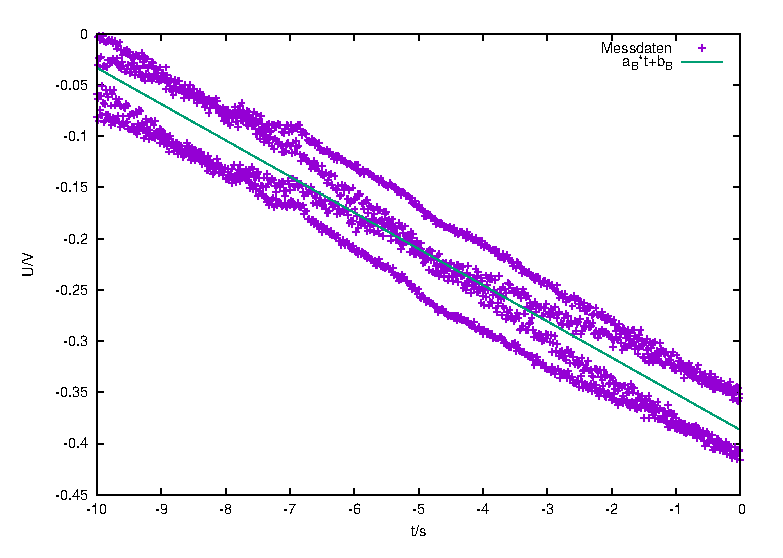
\includegraphics[width=\textwidth]{graphics/fit_Eingangsruhestrom_OVB084.eps}
    \caption{Spannungsverlauf zur Ermittlung des Eingangsruhestroms am
    OV B084, $C=1.5~\mathrm{nF}$}
    \label{fig:ERS_B}
\end{figure}
\begin{figure}[!ht]
    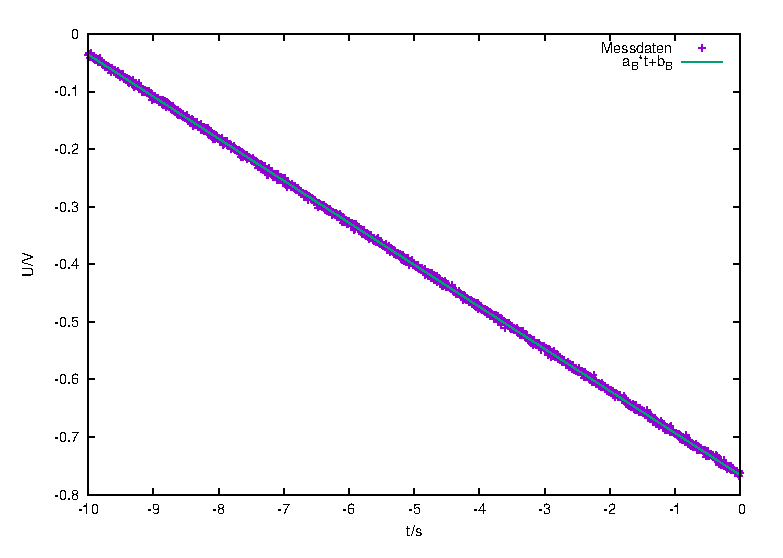
\includegraphics[width=\textwidth]{graphics/fit_Eingangsruhestrom_A109.eps}
    \caption{Spannungsverlauf zur Ermittlung des Eingangsruhestroms am A109,
    $C=4~\mathrm{\mu F}$}
    \label{fig:ERS_A}
\end{figure}

Die dort eingezeichneten Fit-Geraden ergeben jeweils einen Anstieg,
der es ermöglicht, den Strom zu berechnen.
Zur Beurteilung des Fehlers wird für die Kapazitäten ein
recht hoher Rundungsfehler von einer halben Stelle nach Angabe angenommen.

\begin{align*}
    a_B \,&=\, \left(-0.03537\pm 0.00024\right)~\mathrm{\frac{V}{s}}\\
          &=\, -0.03537 \, \left(1\pm0.66\%\right)~\mathrm{\frac{V}{s}}\\
    b_B \,&=\, \left(-0.3868 \pm 0.0014\right)~\mathrm V\\
          &=\, -0.3868 \, \left(1\pm 0.35\%\right)~\mathrm V\\
    C_B \,&=\,1.5~\mathrm{nF}\\
    \Rightarrow
    I_B \,&=\, \left(-53.1\pm2.2\right)~\mathrm{pA}\\
    &=\, -53.1\,\left(1\pm3.99\%\right)~\mathrm{pA}
\end{align*}

\begin{align*}
    a_A \,&=\, \left(-0.073033\pm 0.000020\right)~\mathrm{\frac{V}{s}}\\
          &=\, -0.073033 \, \left(1\pm0.03\%\right)~\mathrm{\frac{V}{s}}\\
    b_A \,&=\, \left(-0.76603 \pm 0.00012\right)~\mathrm V\\
          &=\, -0.76603 \, \left(1\pm 0.02\%\right)~\mathrm V\\
    C_A \,&=\,4~\mathrm{\mu F}\\
    \Rightarrow
    I_A \,&=\, \left(-290\pm40\right)~\mathrm{nA}\\
    &=\, -290\,\left(1\pm12.53\%\right)~\mathrm{nA}
\end{align*}

\section {Auswertung}



\pagebreak
% \section {Quellen}
% \begin{thebibliography}{999}
% \bibitem {WalterHerms} G. Walter und G. Herms, Einführung in die Behandlung von Messfehlern -- Ein Leitfaden für das Praktikum der Physik, Universität Rostock 2006d
% \end{thebibliography}

\section {Anhang}


\end{document}
%sagemathcloud={"zoom_width":100}
